% Na zvoleném českém korpusu vyhodnoťte přesnost a pokrytí pravidel. Diskutujte míru, se kterou je možné generovat gramatické věty, a kvalitu textu (přirozené vyjadřování, nezamýšlené vedlejší efekty).

\section{Evaluation Corpus}

For evaluation, I have constructed my own text corpus. The corpus is composed of texts written by contemporary Czech authors who provided the texts themselves. The corpus is intentionally small as humans did the evaluation, and evaluating a large set of sentences would be expensive.

In selecting the texts, I tried to capture various characteristics of the texts. Thus, the corpus consists of several different literary genres; the narrators are both male and female; I have included texts written in the present and past tense, and I have chosen texts containing different types of speech. (Such as direct speech, semi-direct speech...) Finally, the corpus, of course, includes both first-person and third-person narratives.

In total, the evaluation data consists of 36 different texts composed of 388 sentences. The numbers divided by narratives are captured in chart \ref{fig:eval-input-numbers}.

\begin{figure}[!ht]
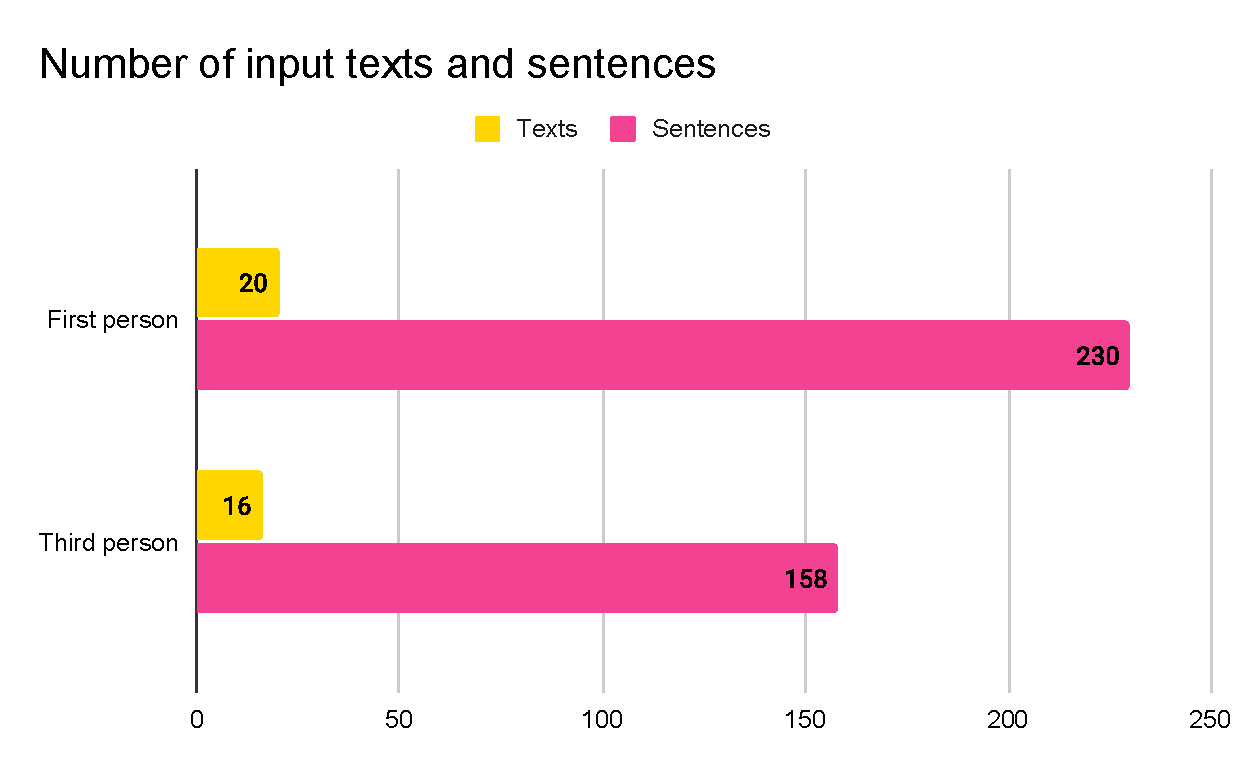
\includegraphics[width=\textwidth]{data/Eval-Input-Numbers.pdf}
\caption{Statistics about the corpus}
\label{fig:eval-input-numbers}
\end{figure}

\section{Annotation Process}

As mentioned in the previous section, human annotators evaluated the sentences manually. The annotators have got: the person the text is converted from, the name of the protagonist, the original text, and the rephrased text. After reading the texts, an annotator could mark one or more statements for each sentence as true.

The possible statements to mark:

\begin{itemize}
	\item The sentence is converted correctly, without grammatical errors, sounds natural, and is unambiguous.
	\item The sentence has lost its unambiguity.
	\item The word order is unnatural, or there are other unnatural sounding elements in the sentence.
	\item The sentence contains grammatical errors.
	\item Some parts of the sentence are converted correctly, and some are not.
	\item The sentence is not converted correctly or not converted at all.
	\item The sentence has not been converted, and that is correct.
\end{itemize}

The evaluation's non-binarity also offers a basic error analysis, which gives us a basis for discussion about the quality of generated texts.

\section{Results}

Based on the marking, I retrieved the results statistics.

As can be seen in figure \ref{fig:eval-total}, most of the sentences were converted correctly, which also includes not converting the sentence at all (about 66\%). Only 17\% of the 388 sentences were converted incorrectly, partially, or entirely. The remaining 17\% are sentences that were converted correctly. However, the conversion damaged the text's quality (naturalness of expression, unambiguity, or grammar).

\begin{figure}[!ht]
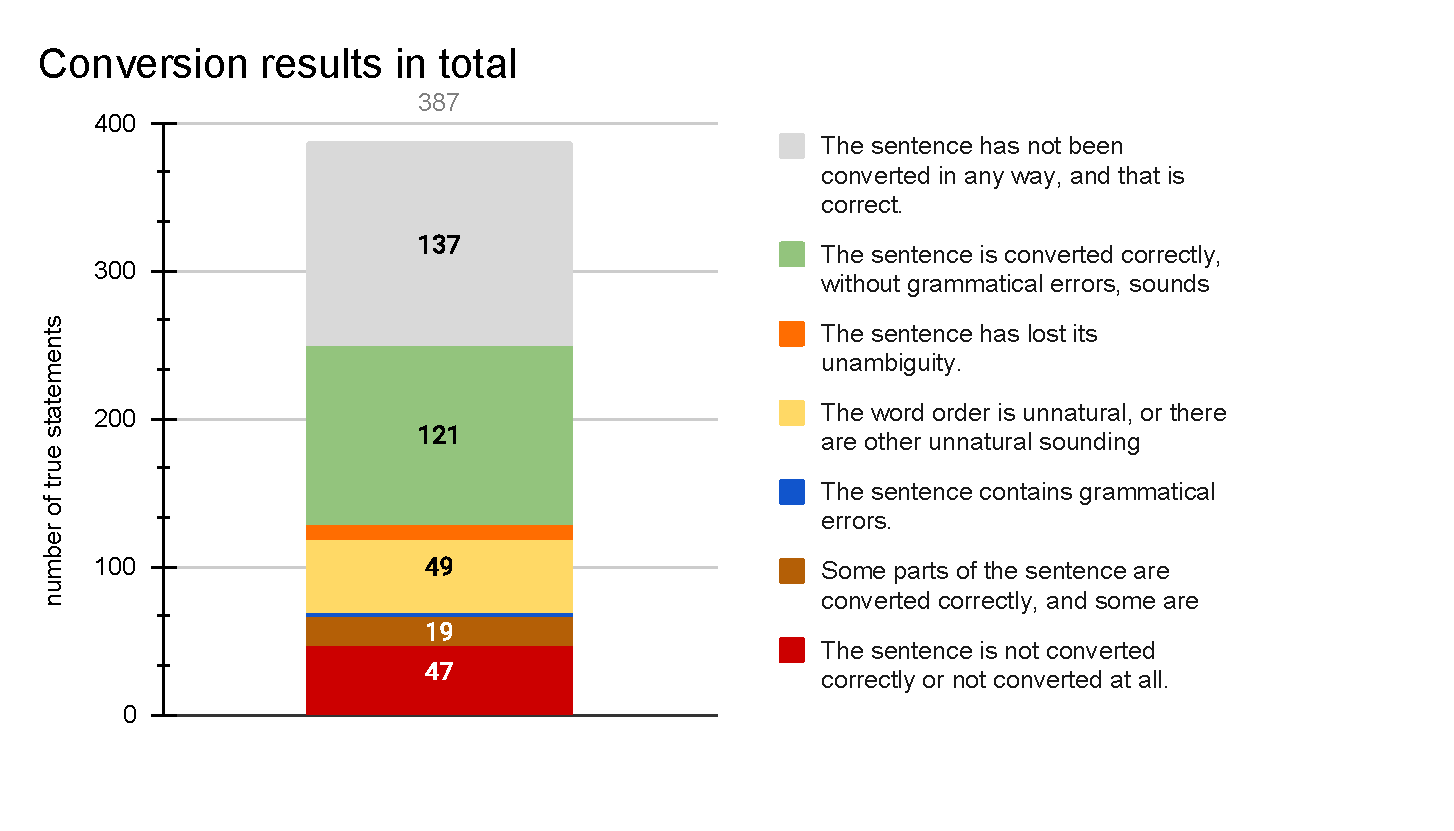
\includegraphics[width=\textwidth]{data/Eval-Total.pdf}
\caption{Results statistics in total}
\label{fig:eval-total}
\end{figure}

Now let us take a look at the results for each narrative mode.

\subsection{First-person to Third-person results}

Figure \ref{fig:eval-first-to-third} shows very good results for the first-person narrative to third-person narrative conversion. Less than 5\% of the sentences were converted partially or completely incorrectly. Moreover, about 82\% of the remaining sentences were converted (or not converted) without any quality loss. The most common problem was unnatural word order.

\begin{figure}[!ht]
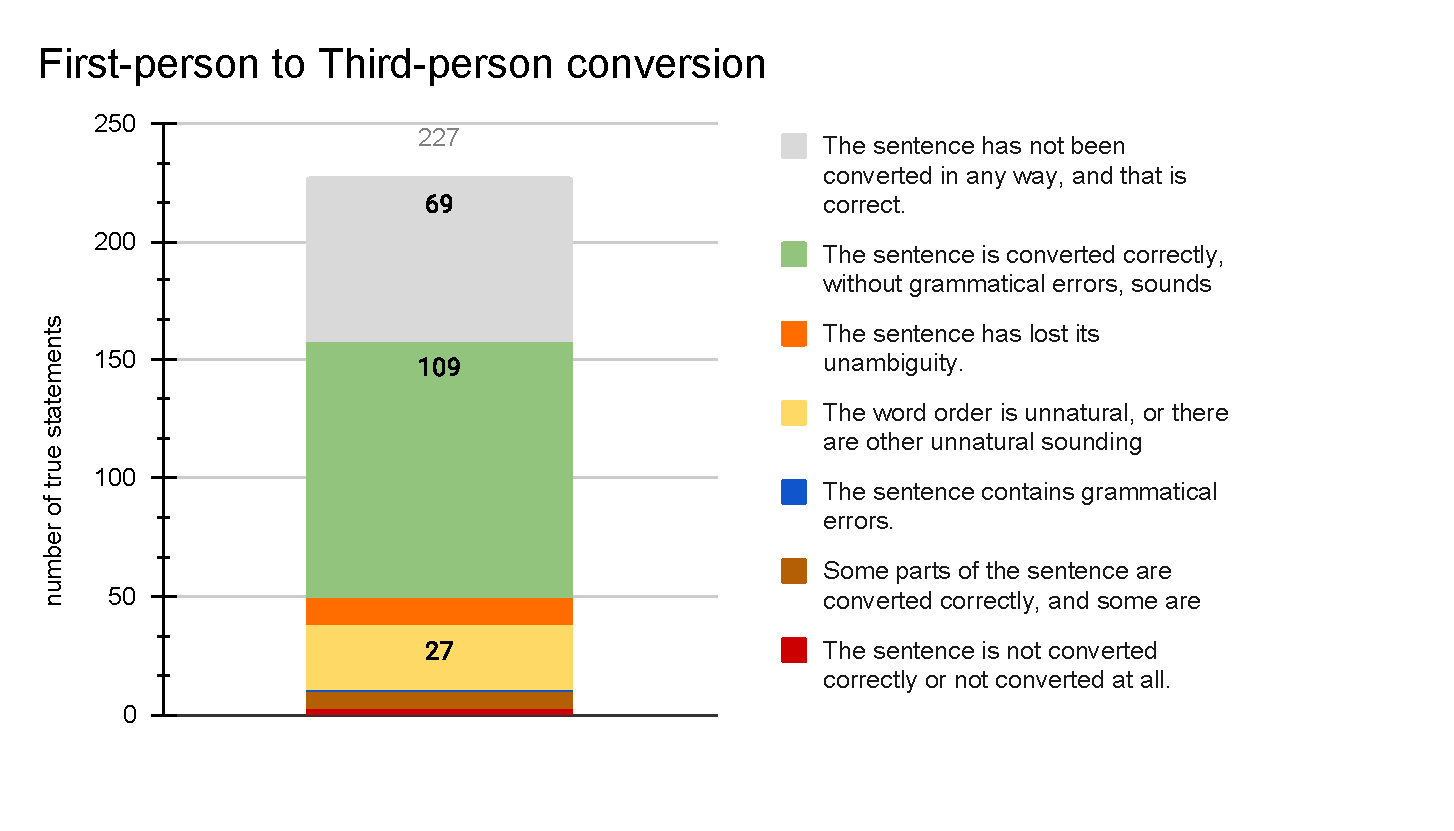
\includegraphics[width=\textwidth]{data/Eval-First-To-Third.pdf}
\caption{Results statistics for first-person to third-person conversion}
\label{fig:eval-first-to-third}
\end{figure}

In Table \ref{tab:example-first}, I show examples of rephrased sentences with the assigned results.

\begin{table}[!ht]
	\caption{Examples of rephrased sentences from first-person to third-person narrative}
	\label{tab:example-first}
		\begin{tabular}{m{5em}|m{11em}|m{11em}}
			result & original sentence & rephrased sentence \\
			\hline
			Correct & Mám sto chutí sebou trhnout a vysvobodit se z doteku jeho horkých prstů, ale vím, že mi to pouta nedovolí, a i kdybych je neměla, zřejmě by na to moje tělo nenašlo sílu. &  Majka má sto chutí sebou trhnout a vysvobodit se z doteku jeho horkých prstů, ale ví, že jí to pouta nedovolí, a i kdyby je neměla, zřejmě by na to její tělo nenašlo sílu. \\
			Ambiguous & \emph{Odvrátila jsem pohled z~ráje a uviděla Evu.} Následovala mě. & \emph{Odvrátila pohled z ráje a uviděla Evu.} Následovala ji. \\
			Unnatural & Byla jednou z mála lidí, se kterou jsem se sblížil. & Byla jednou z mála lidí, se kterou Gabriel se hodně sblížil. \\
			Grammar error & Sdílela se mnou jídlo. & Sdílela se jí jídlo. \\
			Incorrect & Její obličej nerozeznám, ale slyším, že pláče. & Její obličej nerozezná, ale slyším, že pláče. \\
		\end{tabular}
\end{table}


\subsection{Third-person to First-person results}
On the other hand, figure \ref{fig:eval-third-to-first} illustrates quite a different picture. The third-to-first conversion direction delivers poor performance results. Notice that the number of completely incorrect sentences is very high (more than 25\%) even when considering the fact that 68 sentences were not affected by the conversion at all.
The reasons for these poor results are further described in Section \ref{sec:errors}.

\begin{figure}[!ht]
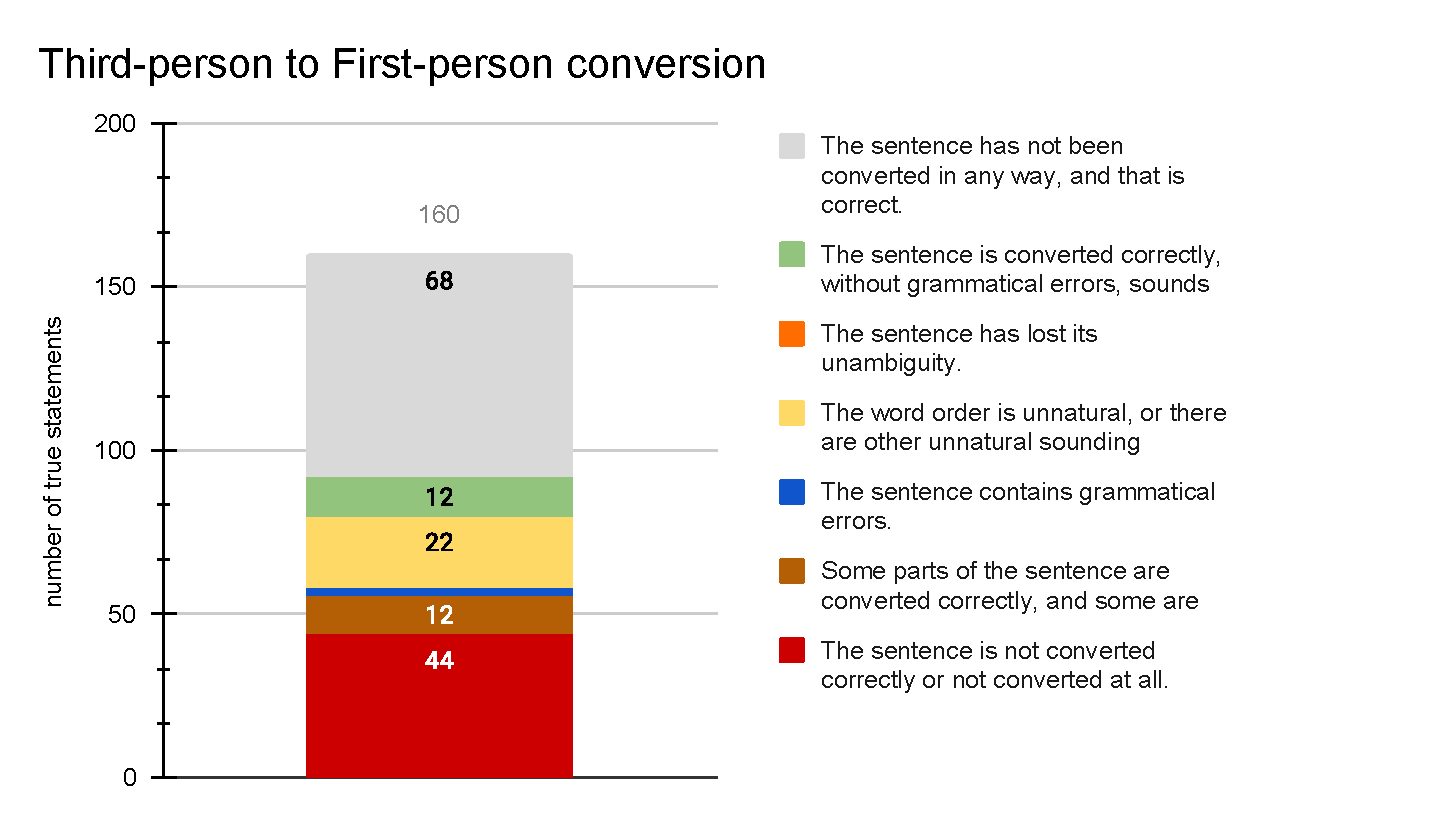
\includegraphics[width=\textwidth]{data/Eval-Third-To-First.pdf}
\caption{Results statistics for third-person to first-person conversion}
\label{fig:eval-third-to-first}
\end{figure}

Examples of the sentences are shown in Table \ref{tab:example-third}.

\begin{table}[!ht]
	\caption{Examples of rephrased sentences from third-person to first-person narrative}
	\label{tab:example-third}
	\begin{flushleft}
		\begin{tabular}{m{5em}|m{11em}|m{11em}}
			result & original sentence & rephrased sentence \\
			\hline
			Correct & Král a královna osaměli. & Král a já jsme osaměli. \\
			Unnatural & Hana se na ni dívala a čekala. & Se na ni jsem dívala a čekala. \\
			Grammar error & Eva byla ráda, že se matka nechala přesvědčit, aby utekly. & Já byla ráda, že se matka nechala přesvědčit, aby jsme utekly. \\
			Incorrect & Hana má pocit, jako by prošvihla nějakou několikaměsíční akci, kde se všichni mezitím seznámili. & Mám pocit, jako by prošvihla nějakou několikaměsíční akci, kde se všichni mezitím seznámili.\\
		\end{tabular}
	\end{flushleft}
\end{table}


\section{Errors and How to Fix Them} \label{sec:errors}

In this section, I provide an error analysis. I examine the causes of the errors and discuss their solvability. The errors are divided into two groups: 1) incorrect conversion and 2) text quality lost.

\subsection{Conversion Errors}

As mentioned in the previous section, most conversion errors come from the third-to-first conversion. Since this direction is much more complicated than the other way, the poorer results are not surprising. In contrast to first-to-third, when converting a text from the third-person narrative, we need to recognize the protagonist who should become the narrator and change all the words whose form depends on this protagonist. This task should be handled by anaphora resolution. Nevertheless, the performance of Aara is poor. Thus, it affects RephrasErIch. The considerable difference between first-to-third and third-to-first results confirms this issue since anaphora resolution is not used in the first-to-third conversion.

A solution to this error is beyond the limits of the tool. Aara would have to be improved or replaced by better performing tool.

\subsection{Text Quality Errors}

\subsubsection{Word order}

Unnatural word order is the most common quality error. It was usually caused by adding or removing words during the conversion. It mostly includes:

\begin{itemize}
	\item \textbf{Adding or removing a subject.} Example: \emph{Adam věří jim to.} The original sentence here was \emph{Věřím jim to.} and the tool added the protagonist's name at the beginning of the sentence. However, the other words should be reordered to sound natural: \emph{Adam jim to věří.}
	\item \textbf{Adding or removing an auxiliary verb.} Example: \emph{Konečně se jsem mohla rozesmát.} The auxiliary verb \emph{jsem} was added to the original sentence \emph{Konečně se mohla rozesmát.}. In Czech, it is natural for reflexive pronoun \emph{se} to come after the auxiliar: \emph{Konečně jsem se mohla rozesmát.}
\end{itemize}

Word order in Czech is not entirely free, but it is variable. It is applied mainly by the role of the sentence members but also by the rhythmic principle and other circumstances. Often, the word order is determined semantically. Their informativeness and expressive dynamics influence the order of the sentence members, and it also depends on the type of sentence. \cite{vlasin-slovnik} This semantic principle would be challenging to implement in the tool. On the other hand, most words remain in the same order after rephrasing, so I believe that semantics has a relatively minor influence on unnaturalness.

Another principle mentioned is the rhythmic principle. The rhythm of a sentence is mainly influenced by the position of unstressed clitics, such as short forms of personal pronouns (\emph{mě, mi, ho, mu...}), reflexive pronouns (\emph{se, si}) or auxiliary verbs (\emph{jsem, bych, by...}). \cite{vlasin-slovnik}

The relative order of clitics is quite precisely defined. Thus, adding a few rules might help the tool generate more natural sentences.


\subsubsection{Prepositions}

Some prepositions in Czech have both vocalized and non-vocalized forms. The vocalized (longer) versions are used mainly for easier pronunciation. Usually, when the word after the preposition begins with the same consonant or a sequence of several consonants. However, it may also depend on other factors, such as rhythm. \cite{vlasin-slovnik}

For instance, let us have a sentence \emph{Táta šel k ní}. Converting the sentence to the first-person narrative, we get \emph{Táta šel k mně}. However, that is unnatural, and it is harder to pronounce -- we would rather write \emph{Táta šel ke mně}. This also applies in vice versa.

Currently, the tool does not change the prepositions when the following word converts. However, this issue would be solvable, at least for cases where the word begins with the same consonant or multiple consonants.


\subsubsection{Proper nouns, unnaturalness, and ambiguity}

When rephrasing, the tool decides in some processes whether to add the proper name of the protagonist instead of the unexpressed subject or pronoun, especially when converting from first to third person. One reason for this addition is to avoid ambiguity. However, this decision is made randomly, leading to the unnaturalness of the text and ambiguity problems.

The \textbf{unnaturalness} occurs when a proper name is inserted in the wrong place in a sentence.

An example may be the following sentence: \emph{Rozhodl jsem se, že půjdu na nákup.} RephrasErIch generated an output: \emph{Rozhodl se, že Adam půjde na nákup.} The sounding would become natural if the proper noun (\emph{Adam}) would stand in the first phrase of the sentence or nowhere. Also, overuse of the name can be unnatural.

In contrast to unnaturalness, \textbf{ambiguity} occurs when a proper name is not inserted. In the first-person narrative, the grammatical person identifies whom the word refers. However, by conversion, we lose this identification. Hence the need to add a proper name to clarify the meaning.

It is a matter of considering where to draw the line between naturalness and ambiguity. Using a proper name in every phrase would lead to perfect unambiguity, but such a sentence would sound highly unnatural. That is the reason why the tool adds the name only with some probability. Nevertheless, it might be helpful to implement a more intelligent decision algorithm, which would consider the position of the phrase in the sentence and further context.

